\chapter{Wireless M-Bus protokol}
Wireless M-Bus je v Evropě perspektivní otevřený standard pro automatické měření, který pracuje v subgi-gaherzovém bezlicenčním pásmu v okolí 868 MHz. Wireless M-Bus se primárně zaměřuje na použití v SRD (Short Range Device) zařízeních pro bezdrátovou komunikaci s měřiči energií, jako jsou: voda, plyn, teplo, elektřina, atd. Měřiče energií, vybavené bezdrátovým rozhraním Wireless M-Bus jsou schopny komunikovat jak se stacionárními, tak i s mobilními čtecími zařízeními. Předpokládá se, že rádiová část měřiče je napájena z baterie a je schopna provozu po dlouhou dobu bez zásahu, tj. bez výměny baterie. Na čtecích zařízeních, ať už stacionární nebo mobilní, není takový požadavek na dobu provozu na baterie a čtecí zařízení mohou být napájena i z externího zdroje.

Wireless M-Bus má svůj původ v rámci norem Meter-Bus. Wireless Meter Bus je bezdrátovou variantou drátového Meter-Bus. To je standard zaměřený na aplikace pro sběr dat měřiče plynu, elektřiny a vody. Sběrnice je specifikována v evropské normě EN 13757~\cite{Norma1}. Tato specifikace je rozdělena do pěti částí (viz Tab.~\ref{TableNorma}), z nichž jedna se zaměřuje na Wireless M-Bus.

\begin{table}[!ht]
\centering
\caption{Popis standardu EN-13757~\cite{WmbusTables}}
\label{TableNorma}
\resizebox{\textwidth}{!}{%
\begin{tabular}{|l|l|}
\hline
{\textbf{Standard}} & \multicolumn{1}{c|}{\textbf{Podrobnosti}} \\ \hline
EN 13757-1 & \begin{tabular}[c]{@{}l@{}}Část 1 standardu definuje výměnu dat, která podrobně popisuje základní \\ komunikaci mezi vodoměry a centrálním sběračem dat. Poskytuje přehled \\ komunikačního systému.\end{tabular}\\ \hline
EN 13757-2 & \begin{tabular}[c]{@{}l@{}}Tato část normy Meter Bus řeší fyzickou a spojovou vrstvu pro fyzický přenos \\ dat pomocí kabelových spojů. Také popisuje protokol používaný pro přenos dat\end{tabular} \\ \hline
EN 13757-3 & \begin{tabular}[c]{@{}l@{}}Část 3  se týká speciální aplikační vrstvy. Ta popisuje standardní aplikační\\  protokol používaný k tomu, aby se zachovala kompatibilita výrobců, což \\ umožňuje zařízení od několika různých dodavatelů působit v jednom systému.\end{tabular} \\ \hline
EN 13757-4 & \begin{tabular}[c]{@{}l@{}}Oddíl 4 popisuje bezdrátový systém. Jedná se o radiový odečet pro provoz v pásmu \\ 868 MHz až 870 MHz . Tato část normy se zabývá fyzickou a linkovou vrstvou pro\\  bezdrátová zařízení.\end{tabular} \\ \hline
EN 13757-5 & \begin{tabular}[c]{@{}l@{}}Tato část adresy předávání. To zahrnuje celou řadu návrhů na předávání datových \\ rámců jako prostředek k překonání problémů souvisejících se pohybují mezi \\ měřičem a sběru dat bodů.\end{tabular} \\ \hline
\end{tabular}}
\end{table}

%%%%%%%%%%%%%%%%%%%%%%%%%%%%%%%%%%%%%%%%%%%%%%%%%=
%%%%%%%%%%%%%%%%%%%%%%%%%%%%%%%%%%%%%%%%%%%%%%%%%=
%%%%%%%%%%%%%%%%%%%%%%%%%%%%%%%%%%%%%%%%%%%%%%%%%=
%%%%%%%%%%%%%%%%%%%%%%%%%%%%%%%%%%%%%%%%%%%%%%%%%=

\section{Princip komunikace}

Bezdrátová komunikace Wireless M-Bus fyzicky probíhá ve 12 kanálech v bezplatném vysílacím pásmu ISM (industrial, scientific and medical) okolo frekvence 868\,MHz (2~kanály\,868,3 a 868,95\,MHz jsou využívány režimem S a T, 10 uživatelem volitelných kanálů 868.03 + n x 0.06\,MHz v režimu R2), přičemž každý z výše uvedených režimů vyžaduje různé požadavky. Těmi například jsou specifikovaný kanál, přesnost frekvence, toleranci přenosové rychlosti atd. Velmi dobrá je stabilita frekvence až 27 let (dle údaje výrobce). V případě použití čtvrtvlné antény (délky 8,2 cm), tak na přímou viditelnost vysílací a přijímacího modulu je komunikační dosah 500 až 600\,m.

Komunikace má hvězdicovitou strukturu, kdy několik měřících jednotek/snímačů přenáší svá naměřená data jedné centrální jednotce, obvykle tvořené koncentrátorem. Ten tedy obvykle slouží pro příjem a shromaždování dat z několika měřících míst, z dále uvedených důvodů nikdy neinicializuje (nezahajuje) vzájemnou komunikaci. Pracuje tedy jako server (Master), tzn. že stále naslouchá a čeká na navázání komunikace měřící jednotkou a jí inicializovaný přenos dat. Ta tedy pracuje jako klient (Slave). V případě nastavené obousměrné komunikace přechází měřič/snímač do přijímacího režimu pouze po krátký čas jím navázané komunikaci. Pouze v tomto momentu může koncentrátor vyslat nějaké jednotce řídící data. Časování je rozdílné pro různé režimy a je přesně specifikováno ve standardu.

Adresování ve Wireless M-Bus sběrnici je převzato z klasické drátové verze M-BUSu. Zde však pouze klientské jednotky (měřiče/snímače) mají přidělenou adresu a využívají ji jak při příjmu, tak při vysílání. Každý koncentrátor by měl obsahovat tabulku adres, se kterými může komunikovat, resp. od kterých má přijímat data. Tato tabulka se obvykle vytváří automaticky během instalace/registrování nové jednotky do sítě. Samozřejmě je možné se obejít i bez ní, ale pak lze přijímat všechny snímače či měřiče v dosahu. Toho se dá využít jen v malých sítích. 

%%%%%%%%%%%%%%%%%%%%%%%%%%%%%%%%%%%%%%%%%%%%%%%%%=
%%%%%%%%%%%%%%%%%%%%%%%%%%%%%%%%%%%%%%%%%%%%%%%%%=
%%%%%%%%%%%%%%%%%%%%%%%%%%%%%%%%%%%%%%%%%%%%%%%%%=
%%%%%%%%%%%%%%%%%%%%%%%%%%%%%%%%%%%%%%%%%%%%%%%%%=

\section{Režimy přenosu}
Nejdůležitější vlastností technologie WM-Bus je možnost bateriového napájení měřicích zařízení. V případě bezdrátové komunikace je výhodné například měřiče tepla nebo vodoměry napájet jen bateriově a tím eliminovat jakoukoliv nutnost pokládání kabelů. To ale znamená velmi omezenou spotřebu elektrické energie, aby baterie vydržely co nejdéle, alespoň několik let. V současné době v případě napájení modulu lze dosáhnout životnost na jednu baterii až 12~let~\cite{CidloBonega,CidloWeptech}. Aby to však bylo možné, řízení přenosu dat musí co nejčastěji přecházet do nízkopříkonového stavu (sleep mode) a vysílat data jen v nutných případech v co nejkratších časových slotech. Proto také centrální zařízení (koncentrátor), který obvykle slouží pro příjem a shromaždování dat z několika měřících míst, nikdy nesmí inicializovat vzájemnou komunikaci.

Protokol podporuje několik režimů přenosu, lišících se dle požadavků na konkretní aplikaci. Je definováno několik režimů označených jako S, T a R představující 3 různé různé přenosové rychlosti, které se dále dělí na režim 1 a 2, což značí jednosměrný či obousměrný přenos dat. U některých zařízení mohou být doplněny o režimy N, C a F. Tyto režimy jsou shrnuty v Tab.~\ref{TableRezimy}.

\begin{table}[!ht]
\centering
\caption{Režimy přenosu WM-Bus protokolu~\cite{WmbusTables}}
\label{TableRezimy}
\resizebox{\textwidth}{!}{%
\begin{tabular}{|c|l|l|l|l|l|}
\hline
\textbf{Mód} & \multicolumn{1}{c|}{\textbf{Mód přenosu}} & \multicolumn{1}{c|}{\textbf{Směr}} & \multicolumn{1}{c|}{\textbf{Frekvence}} & \multicolumn{1}{c|}{\textbf{Kódování}} & \multicolumn{1}{c|}{\textbf{Rychlost}} \\ \hline
S & Stacionární & \begin{tabular}[c]{@{}l@{}}Jednosměrný,\\ i obousměrný\end{tabular} & 868\,MHz & Manchester & 32768\,kbps \\ \hline
T & Častý vysílací & \begin{tabular}[c]{@{}l@{}}Jednosměrný,\\ i obousměrný\end{tabular} & 868\,MHz & \begin{tabular}[c]{@{}l@{}}Manchester \\  a 3 z 6\end{tabular} & 100\,kbps \\ \hline
R & Častý přijímací & \begin{tabular}[c]{@{}l@{}}Jednosměrný,\\ i obousměrný\end{tabular} & 868\,MHz & Manchester & 4.8\,kbps \\ \hline
N & Úzkopásmový & \begin{tabular}[c]{@{}l@{}}Jednosměrný,\\ i obousměrný\end{tabular} & 169\,MHz & NRZ &  \\ \hline
C & Kompaktní & \begin{tabular}[c]{@{}l@{}}Jednosměrný,\\ i obousměrný\end{tabular} & 868\,MHz & Manchester & 50\,kbps \\ \hline
F & \begin{tabular}[c]{@{}l@{}}Častý vysílací \\ i přijímací mód\end{tabular} & Obousměrný & 433\,MHz & NRZ &  \\ \hline
\end{tabular}}
\end{table}


V	módu T měřič samostatně odesílá data, buď periodicky nebo aperiodicky (když jsou k dispozici). Pro přenos rámce z měřiče k dalším zařízením je použita přenosová rychlost 100 kbps s kódováním 3 z 6, zatímco komunikace v opačném směru má přenosovou rychlost 32768 kbps a kódování je použito Manchester. Submód T1 je definován jako jednosměrná komunikace, při které měřič nevyžaduje potvrzení od příjemce o přijatém rámci. Měřič odešle data a přepne se do úsporného režimu. Zatímco submód T2 je definován jako obousměrná komunikace. Měřič po odeslání rámce krátkou dobu vyčkává na potvrzení od příjemce. Pokud měřič neobdrží odpověď přepne se do úsporného režimu. Pokud ve stanoveném čase příjemce odpoví, naváže se obousměrná komunikace mezi měřičem a koncentrátorem.


V	módu R měřič samostatně neodesílá změřená data, ale vyčkává na výzvu od koncentrátoru. Měřič je v úsporném režimu a pravidelných úsecích se periodicky probouzí do režimu přijmu a očekává rámec. Když není přijat žádný validní wake-up rámec, měřič se přepne zpět do úsporného režimu. V	opačném případě se naváže obousměrná komunikace mezi měřičem a koncentrátorem.


Mód S je určen pro jednosměrnou nebo obousměrnou komunikaci mezi pevnými nebo mobilními zařízeními. Centrální frekvence tohoto módu je 868,3\, MHz s dobou provozu 0,02\,\% za hodinu. Přenosová rychlost je pro tento mód 32,768\,kbps. Pro operační mód S jsou definovány tři submódy: S1, S1-m a S2. Submód S1 lze použít pro jednosměrnou komunikaci nevyžadující potvrzení o přijetí rámce a je určen pro aplikace, kdy se vysílá několikrát za den ke statickému přijímači. Pro kódování používají všechny submódy módu S kódování Manchester.  
Submód S1-m je modifikací submódu S1 pro komunikaci mezi čidlem a koncentrátorem, zasílaný rámec obsahuje zkrácenou hlavičku.
Submód S2M podporuje oboustranou komunikaci v kontinuálních cyklech bez nutnosti probouzet zařízení.

V režimech S, T a R je každý bajt vysílán s nejvíce důležitým bitem na prvním místě.


Princip obousměrné komunikace v módech T2 a S2 je znázorněn na Obr.~\ref{ObrazekObousmerny}:
\colorbox[rgb]{1,0,0}{PREKRESLIT POKUD ZUSTANE} 

\begin{figure}[!ht]
 \begin{center}
    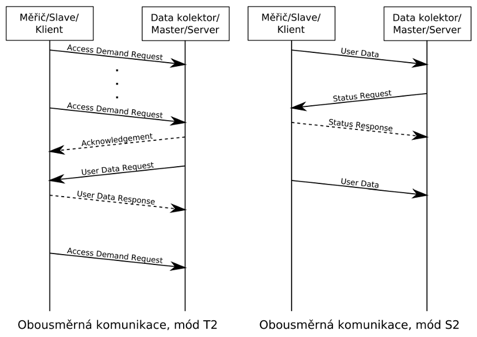
\includegraphics[scale=0.8]{obrazky/wmbus_obousmerne}
  \end{center}
  \caption{Princip obousměrné komunikace v módech T1 a S1}
	\label{ObrazekObousmerny}
\end{figure}

 V obousměrném vysílacím módu měřič s periodou několika sekund vysílá krátkou zprávu se svým ID a pokud koncentrátor na tuto výzvu odpoví, zahájí se obousměrná komunikace.


%%%%%%%%%%%%%%%%%%%%%%%%%%%%%%%%%%%%%%%%%%%%%%%%%=
%%%%%%%%%%%%%%%%%%%%%%%%%%%%%%%%%%%%%%%%%%%%%%%%%=
%%%%%%%%%%%%%%%%%%%%%%%%%%%%%%%%%%%%%%%%%%%%%%%%%=
%%%%%%%%%%%%%%%%%%%%%%%%%%%%%%%%%%%%%%%%%%%%%%%%%=


\section{Struktura zasílaných dat}
Komunikace probíjá následovně: nadřazené aplikace realizující aplikační vrstvu standardu M-Bus vyšlou svá data do RF modemu v podobě datové jednotky, která je zobrazena v Tab.~\ref{PaketWm1}:

\begin{table}[!ht]
\centering
\begin{tabular}{ccc}
1 Bajt & 1 Bajt & n Bajtů \\ \hline
\multicolumn{1}{|c|}{Length} & \multicolumn{1}{c|}{CI} & \multicolumn{1}{c|}{AppLayer} \\ \hline
\end{tabular}
\caption{Formát datové jednotky~\cite{FormatDatoveJednotky}}
\label{PaketWm1}
\end{table}

Komunikační modul pracující jako modem dle požadavků standardu Wireless M-Bus automaticky přidá následující pole:

\begin{itemize}
	\item Řídicí pole.
\item Označení výrobce dle~\cite{WmbusVendors}.
\item Unikátní komunikační adresy založené parametrech uložených v paměti modulu.
\item Případně se ještě na závěr přidá informace o síle přijímaného signálu RSSI.
\end{itemize}



\begin{table}[!ht]
\centering
\begin{tabular}{ccccccc}
1 Bajt & 1 Bajt & 2 Bajty & 6 Bajtů & 1 Bajt & n Bajtů & 1 Bajt \\ \hline
\multicolumn{1}{|c|}{Legth} & \multicolumn{1}{c|}{C} & \multicolumn{1}{c|}{ManID} & \multicolumn{1}{c|}{Address} & \multicolumn{1}{c|}{CI} & \multicolumn{1}{c|}{AppLayer} & \multicolumn{1}{c|}{RSSI} \\ \hline
\end{tabular}
\caption{Formát datové jednotky protokolu Wireless M-Bus~\cite{FormatDatoveJednotky}}
\label{PaketWm2}
\end{table}

Takovýto paket se pak zašifruje (obvykle algoritmem AES-128) a přenáší se vzduchem. V případě, že se realizuje jen bezdrátové tunelování přenosu mezi dvěma Wireless M-Bus modemy, je povolen i režim bez zasílání adresy a jí přidružených informacích o měřící jednotce. Rámec se pak výrazně zjednoduší a jeho struktura je zobrazena v Tab.~\ref{PaketWm3}.

			
			\begin{table}[!ht]
\centering
\begin{tabular}{cccc}
1 Bajt & 1 Bajt & n Bajtů & 1 Bajt \\ \hline
\multicolumn{1}{|c|}{Legth} & \multicolumn{1}{c|}{CI} & \multicolumn{1}{c|}{AppLayer} & \multicolumn{1}{c|}{RSSI} \\ \hline
\end{tabular}
\caption{Zkrácený formát datové jednotky~\cite{FormatDatoveJednotky}}
\label{PaketWm3}
\end{table}
			
Obsah pole AppLayer je již dán aplikační hladinou definovanou ve standardu M-Bus, které se používá jako mechanizmus komunikace z linkové vrstvy do vyšších protokolových vrstev, a je tedy shodný s obsahem pro klasický drátový M-Bus přenos.  Data následující za polem Cl jsou již závislá na aplikační vrstvě M-Bus. Komunikace mezi měřící jednotkou a RF modemem či mezi koncentrátorem a RF modem obvykle probíhá prostřednictvím sériového přenosu UART, například s využitím RS-232, RS-485 či USB.



%%%%%%%%%%%%%%%%%%%%%%%%%%%%%%%%%%%%%%%%%%%%%%%%%=
%%%%%%%%%%%%%%%%%%%%%%%%%%%%%%%%%%%%%%%%%%%%%%%%%=
%%%%%%%%%%%%%%%%%%%%%%%%%%%%%%%%%%%%%%%%%%%%%%%%%=
%%%%%%%%%%%%%%%%%%%%%%%%%%%%%%%%%%%%%%%%%%%%%%%%%=

\newpage


\section{Popis jednotlivých vrstev}

Norma EN 13757-4 specifikuje fyzickou a linkovou vrstvu. Na ně následně navazuje aplikační vrstva, která je shodná s původním M-Bus protokolem.

\subsection{Fyzická vrstva Wireless M-Bus}
Fyzická vrstva definuje jak mají být bity kódovány a vysílány, tedy radiofrekvenční charakteristiky a radiofrekvenční parametry. Fyzická vrstva je realizována hardwarem, případně v kombinaci s firmwarem daného hardware.

Wireless M-Bus dle normy ČSN~EN~13757-4~\cite{Norma4} využívá tři pásma pro tři různé módy komunikace: 868,3\,MHz pro módy Sx, 868,95\,MHz pro módy Tx a 868,33\,MHz pro mód R2 jsou definovány tři různé operační módy komunikace. Všechny tři módy používají modulaci 2-FSK, tedy dvoustavovou frekvenční modulaci. Pro některé módy jsou některé parametry fyzické vrstvy stejné, proto je fyzické zařízení schopné s nezměněným hardwarem komunikovat v různých operačních módech.


\subsubsection{Kódování používaná ve Wireless M-Bus}
Wireless M-Bus definuje dvojí možné kódování: 
\begin{itemize}
	\item kódování Manchester,
	\item kódování 3 ze 6. 
\end{itemize}

Kódování Manchester (viz Obr. \ref{ObrazekManechester}) slučuje datový a hodinový signál do jediného signálu. Toto kódování se krom bezdrátových přenosů používá i v sítích LAN, konkrétně v síti Ethernet. Výhodou kódu Manchester je konstantní střední hodnota takového signálu, která je 50\,\% z maximální hodnoty. Náběžné hrany ohraničují jeden bit dat a sestupné hrany určují kód Manchester. Logická jednička je reprezentována náběžnou hranou a logická nula hranou sestupnou. Pokud nejsou vysílána žádná data, výstup kódování Manchester je hodinový signál. Nevýhodou použití Manchester kódování je to, že na přenos jednoho bitu informace je potřeba dvou hodinových taktů.

				\begin{figure}[!ht]
 \begin{center}
    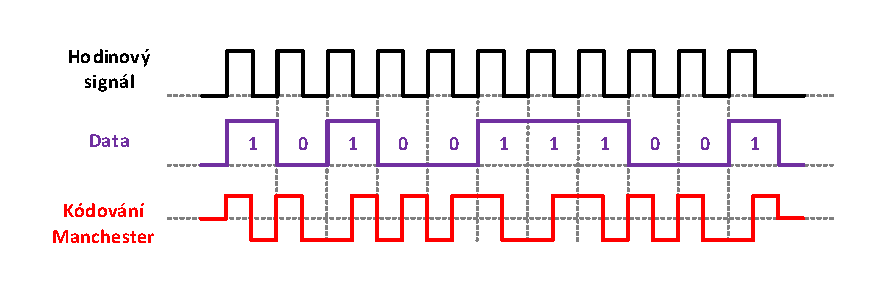
\includegraphics[scale=0.3]{obrazky/wmbus_manchester}
  \end{center}
  \caption{Princip kódování Manchester \cite{Manchester} \colorbox[rgb]{1,0,0}{PŘEKRESLIT}}
	\label{ObrazekManechester}
\end{figure}


Princip kódování 3 ze 6 spočívá v tom, že každé 4 bity (nibble) jsou zakódovány jako 6ti bitová data, přičemž zakódované slovo obsahuje stejné množství nul a jedniček. Zároveň v kódu musí být alespoň dvě změny, tzn. není možné použít \uv{000111} nebo \uv{111000}. Takto zakódovaná data jsou přenášené s nejvýznamnějším bitem jako prvním. Toto kódování by mělo být aplikováno při použití módu častého vysílání (módy T1 a T2) a při komunikaci měřiče s koncentrátorem. Koncentrátor může odpovědět měřiči zprávou kódovanou kódováním Manchester.


\begin{table}[!ht]
\centering
\caption{Tabulka kódování 3 ze 6 \cite{WMencodeing}}
\begin{tabular}{|c|c|c|c|c|}
\hline
\textbf{NRZ kód} & \textbf{Desítkově} & \textbf{3 ze 6} & \textbf{Desítkově} & \textbf{Počet změn v kódu} \\ \hline
0                & 0                  & 10110               & 22                 & 4                          \\ \hline
1                & 1                  & 1101                & 13                 & 3                          \\ \hline
10               & 2                  & 1110                & 14                 & 2                          \\ \hline
11               & 3                  & 1011                & 11                 & 3                          \\ \hline
100              & 4                  & 11100               & 28                 & 2                          \\ \hline
101              & 5                  & 11001               & 25                 & 3                          \\ \hline
110              & 6                  & 11010               & 26                 & 4                          \\ \hline
111              & 7                  & 10011               & 19                 & 3                          \\ \hline
1000             & 8                  & 101100              & 44                 & 3                          \\ \hline
1001             & 9                  & 100101              & 37                 & 4                          \\ \hline
1010             & 10                 & 100110              & 38                 & 3                          \\ \hline
1011             & 11                 & 100011              & 35                 & 2                          \\ \hline
1100             & 12                 & 110100              & 52                 & 3                          \\ \hline
1101             & 13                 & 110001              & 49                 & 2                          \\ \hline
1110             & 14                 & 110010              & 50                 & 3                          \\ \hline
1111             & 15                 & 101001              & 41                 & 4                          \\ \hline
\end{tabular}
\end{table}

\subsection{Linková vrstva Wireless M-Bus}

Linková vrstva poskytuje rozhraní mezi fyzickou a aplikační vrstvou. Její hlavní funkce jsou:
\begin{itemize}
	\item Poskytování služeb převádějících data mezi fyzickou a aplikační vrstvou.
	\item Generování CRC pro odchozí zprávy.
	\item Detekování CRC chyb v příchozích zprávách.
	\item Poskytování adresování fyzické vrstvy.
	\item Kontrola ACK u obousměrných přenosů.
	\item Vytváření rámců.
	\item Kontrola chyb rámců v příchozích zprávách.
\end{itemize}

Rámec linkové vrstvy se skládá z bloků dat. Každý blok dat obsahuje 16bitové CRC pole.  První blok má pevnou délku 12 bajtů a obsahuje L, C, M a A pole.

\subsubsection{L-Pole}
\begin{itemize}
	\item Určuje velikost přenášecných dat, ale bez samotného L-pole a kontrolního součtu.	
\end{itemize}

\subsubsection{C-Pole}
\begin{itemize}
	\item Identifikuje typ rámce.
	\item Používá se pro zasílání základních příkazů.
\end{itemize}

\subsubsection{M-Pole}
\begin{itemize}
	\item Obsahuje identifikaci výrobce zařízení.
	\item Je kódováno jako třípísmenný kód.
	\item Znak je kódován jako 5 bitů, které se získávají z ASCII kódu písmena po odečtení 0x40. Nejvý-znamnější bit (MSB) je nula.
\end{itemize}

\subsubsection{A-Pole}
\begin{itemize}
	\item Obsahuje 6 bajtu určující adresu zařízení.
	\item U rámců SEND a REQUEST je zde adresa vysílajícího zařízení, u rámců CONFIRM a RESPONSE je zde adresa zařízení, které je paket určen.
\end{itemize}

\subsubsection{Cl-Pole}
\begin{itemize}
	\item Určuje typ přenášených dat.
\end{itemize}



\subsubsection{CRC}
\begin{itemize}
	\item CRC obsahuje kontrolní součet pro kontrolu správnosti přenosu. 
	\item Jako kontrolní polynom se dle specifikace používá x\textsuperscript{16} + x\textsuperscript{13} + x\textsuperscript{12} + x\textsuperscript{11} + x\textsuperscript{10} + x\textsuperscript{8} +\textsuperscript{6} + x\textsuperscript{5} + x\textsuperscript{2} + 1.
\end{itemize}


%%%%%%%%%%%%%%%%%%%%%%%%%%%%%%%%%%%%%%%%%%%%%%%%%%%%%%%%%%%%%%%%%%%%%%%%%%%%%%%%%%%%%%%%%%
%%%%%%%%%%%%%%%%%%%%%%%%%%%%%%%%%%%%%%%%%%%%%%%%%%%%%%%%%%%%%%%%%%%%%%%%%%%%%%%%%%%%%%%%%%
%%%%%%%%%%%%%%%%%%%%%%%%%%%%%%%%%%%%%%%%%%%%%%%%%%%%%%%%%%%%%%%%%%%%%%%%%%%%%%%%%%%%%%%%%%
%%%%%%%%%%%%%%%%%%%%%%%%%%%%%%%%%%%%%%%%%%%%%%%%%%%%%%%%%%%%%%%%%%%%%%%%%%%%%%%%%%%%%%%%%%

\section{Šifrování dat}

Pro šifrování přenášených dat se v protokolu Wireless M-Bus používají tři šifrovací algoritmy:
\begin{itemize}
	\item DES bez inicializačního vektoru,
	\item DES s inicializačním vektorem a
	\item AES s inicializačním vektorem.
\end{itemize}

Šifrování DES dnes již není moc využiváne, je již nedostačující a zastaralé. Drtivá většina dnešních zařízení umožnujících šifrovaný přenos využívají šifrování AES, konkrétně verzi AES128 CBC.

\subsection{Šifrovací algoritmus DES}
\colorbox[rgb]{1,0,0}{fakt jen strucne}

\subsection{Šifrovací algoritmus AES}
\colorbox[rgb]{1,0,0}{obecny popis sifry, jak to funguje, kde se to vzalo, proc je to tak super}


\subsection{Určení šifrovaných dat}
\colorbox[rgb]{1,0,0}{neco malo jak se poznaji sifrovana data - bude castecne }

\colorbox[rgb]{1,0,0}{duplicitni s popisem pole SignatureField nebo }

\colorbox[rgb]{1,0,0}{ConfigurationWord v obecnem popisu telegramu.}


\subsection{Módy šifrování AES}
\colorbox[rgb]{1,0,0}{rozepsat mody sifrovani EBC, CTR, a hlavne poradne CBC.}

\colorbox[rgb]{1,0,0}{demonstrovat provazanost na specifiakce (mod5)}

\subsection{Šifrovací klíč}
\colorbox[rgb]{1,0,0}{...kecy ke klíčům...}

\subsection{Inicializační vektor}
Inicializační vektor má délku 16 Bajtů (128 bitů, odtud označení AES128) a je tvořený dynamicky z nešifrovaných bajtů způsobem popsaným v Tab.~\ref{TabulkaInicializacniVektor}:
\begin{figure}[!ht]
 \begin{center}
    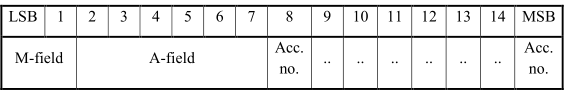
\includegraphics[scale=0.9]{obrazky/sifrovani_vektor}
  \end{center}
  \caption{Formát inicializačního vektoru \colorbox[rgb]{1,0,0}{PREKRESLIT}}
	\label{TabulkaInicializacniVektor}
\end{figure}

První 2 bajty obsahují přidělené identifikační údaje výrobce, další čtyři obsahují sériové číslo daného zařízení, následující dva obsahují verzi zařízení a zbylých osm Bajtů je tvořeno opakováním se přístupového čísla. Vzhledem k faktu, že přístupové číslo se s každým vysláním telegramu změní, je nutné inicializační vektor přepočítat pro každý přijatý paket. Tím je zajištěna dynamičnost šifrování danou metodou.

\subsection{Princip dešifrování}

\colorbox[rgb]{1,0,0}{popsat jak se to desifruje, propojit s ukazkama:}

 \colorbox[rgb]{1,0,0}{desifrovani zminene u knihovny PyCrypto, pripadne pod diagramem s aplikaci}


\subsection{Kontrola rozšifrování dat}
Ke kontrole správnosti dešifrovaných dat slouží definovaná počáteční sekvence dat. U algoritmu DES začínají dešifrovaná data dvěma bajty obsahujícími datum a čas. Pro algoritmus AES jsou první dva bajty šestnáckové a oba obsahují znak 2F.



















